\documentclass[12pt, twoside]{article}
\usepackage[francais]{babel}
\usepackage[T1]{fontenc}
\usepackage[latin1]{inputenc}
\usepackage[left=5mm, right=5mm, top=3mm, bottom=3mm]{geometry}
\usepackage{float}
\usepackage{graphicx}
\usepackage{array}
\usepackage{multirow}
\usepackage{amsmath,amssymb,mathrsfs}
\usepackage{textcomp}
\pagestyle{empty}
\usepackage{soul}
\usepackage{eurosym}
\usepackage{lscape}

\begin{document} 
 


\begin{flushleft}
NOM PRENOM: \ldots \ldots \ldots \ldots \ldots \ldots \ldots \ldots \ldots
 \end{flushleft}


\begin{center}
{\fbox{$6^{e}\ldots$ \qquad \qquad \textbf{\Large{Devoir surveill� 6 }}
\qquad \qquad 11/05/2011}}
\end{center}


\medskip
 

\textit{L'exercice 1 se fait sur la photocopie. La feuille de l'exercice 5 est �
coller sur votre feuille pr�par�e.}

\medskip


\ul{\textbf{Exercice 1:}} \textit{(3 points)}



\begin{tabular}{cc}
\begin{minipage}{13cm}
\begin{enumerate}
  \item Donner les longueurs �gales.
  
  \ldots \ldots \ldots \ldots \ldots \ldots \ldots \ldots \ldots \ldots \ldots
  \ldots \ldots \ldots \ldots \ldots \ldots \ldots  \ldots \ldots \ldots 
  
  \item Faire une phrase en utilisant le mot ``milieu''.
  
  \ldots \ldots \ldots \ldots \ldots \ldots \ldots \ldots \ldots \ldots \ldots
  \ldots \ldots \ldots \ldots \ldots \ldots \ldots  \ldots  \ldots \ldots 
  
  
  \item Placer sur la figure le point K milieu de [GB].
\end{enumerate}
\end{minipage}
&
\begin{minipage}{5cm}
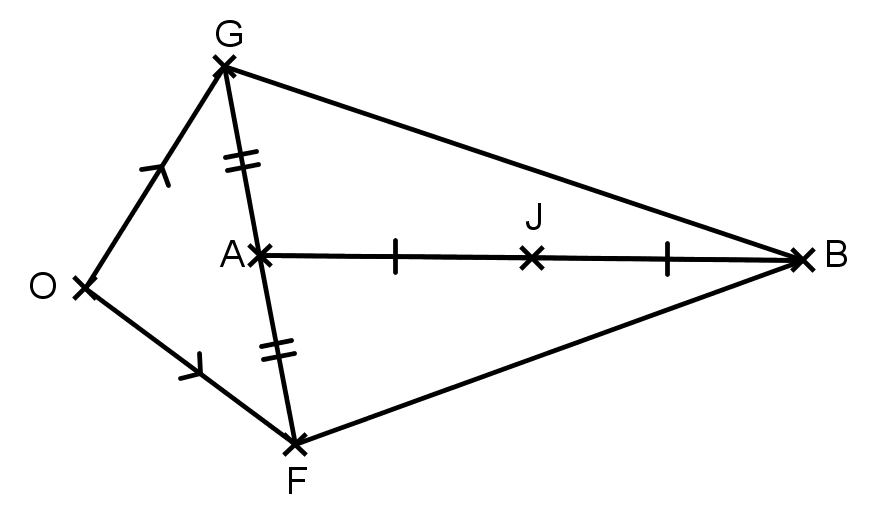
\includegraphics[width=5cm]{images/ex1.png}
\end{minipage}
\end{tabular}

\bigskip


\ul{\textbf{Exercice 2:}} \textit{(2,5 points)}


\begin{tabular}{cc}
\begin{minipage}{12cm}

\begin{enumerate}
  \item Comment s'appelle le segment [HG?]?
  
  \item Comment s'appelle le segment [DE]?

  \item Comment s'appelle la partie du cercle tra��e en pointill�s?
  \item Comment s'appelle le point D?
  \item Comment s'appelle le segment [CF]?
\end{enumerate}
\end{minipage}
&
\begin{minipage}{6cm}
\begin{center}
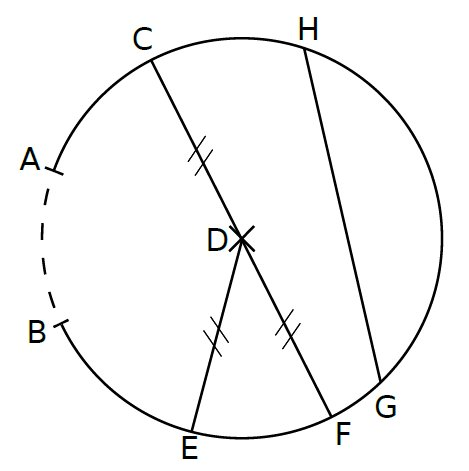
\includegraphics[width=45mm]{images/ex2.jpg}
\end{center}
\end{minipage}
\end{tabular}


\bigskip


\ul{\textbf{Exercice 3:}} \textit{(3,5 points)}

\begin{tabular}{cc}
\begin{minipage}{10cm}
\begin{enumerate}
  \item Construire un triangle GHI tel que GH=8cm, HI=6cm et GI=7cm.
  \item Construire la figure ci-contre en vraie grandeur.
  
 
\end{enumerate}
\end{minipage}
&
\begin{minipage}{8cm}
\begin{center}
 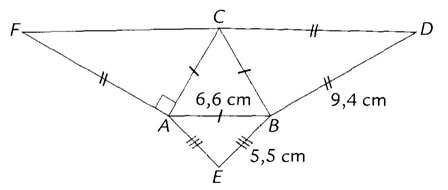
\includegraphics[width=70mm]{images/ex3.png}
 \end{center}
\end{minipage}
\end{tabular}



\bigskip


\ul{\textbf{Exercice 4:}} \textit{(3 points)}


\begin{enumerate}
  \item Tracer un segment [LU] tel que LU=3,6cm.
  \item Tracer la m�diatrice (d) de [LU]. Placer un point M sur la droite (d)
  tel que ML=5cm.
  \item Quelle est la nature du triangle MLU? Justifier votre r�ponse.
\end{enumerate}

\bigskip


\ul{\textbf{Exercice 5:}} \textit{(2,5 points)}


\enskip

La figure ci-contre repr�sente un terrain de P�tanque. 1 m�tre est repr�sent�
par 1 cm.
 

\begin{enumerate}
  \item Marc doit lancer le cochonnet entre 6 m et 9m. Colorer en bleue la
  zone o� il doit lancer le cochonnet.
  \item Apr�s avoir tir�, le cochonnet se trouve � moins de 4 m�tres de John.
  Colorer en vert la zone o� se trouve le cochonnet.
  
\end{enumerate}



\bigskip


\ul{\textbf{Exercice 6:}} \textit{(5,5 points)}

\enskip


Le dessin ci-contre a �t� r�alis� � main lev�e mais il a �t� bien cod�.

\enskip


\begin{tabular}{cc}
\begin{minipage}{12cm}
\begin{enumerate}
  \item Ecrire un programme de construction de cette figure.
  \item Construire cette figure.
  \item Citer deux points de la figure �quidistants de A et B. Justifier.
  \item Quelle est la m�diatrice du segment [AB]? Justifier.
\end{enumerate}
\end{minipage}
&

\begin{minipage}{6cm}

\end{minipage}
\end{tabular}



\pagebreak




\begin{landscape}

\begin{center}
\begin{tabular}{cc}
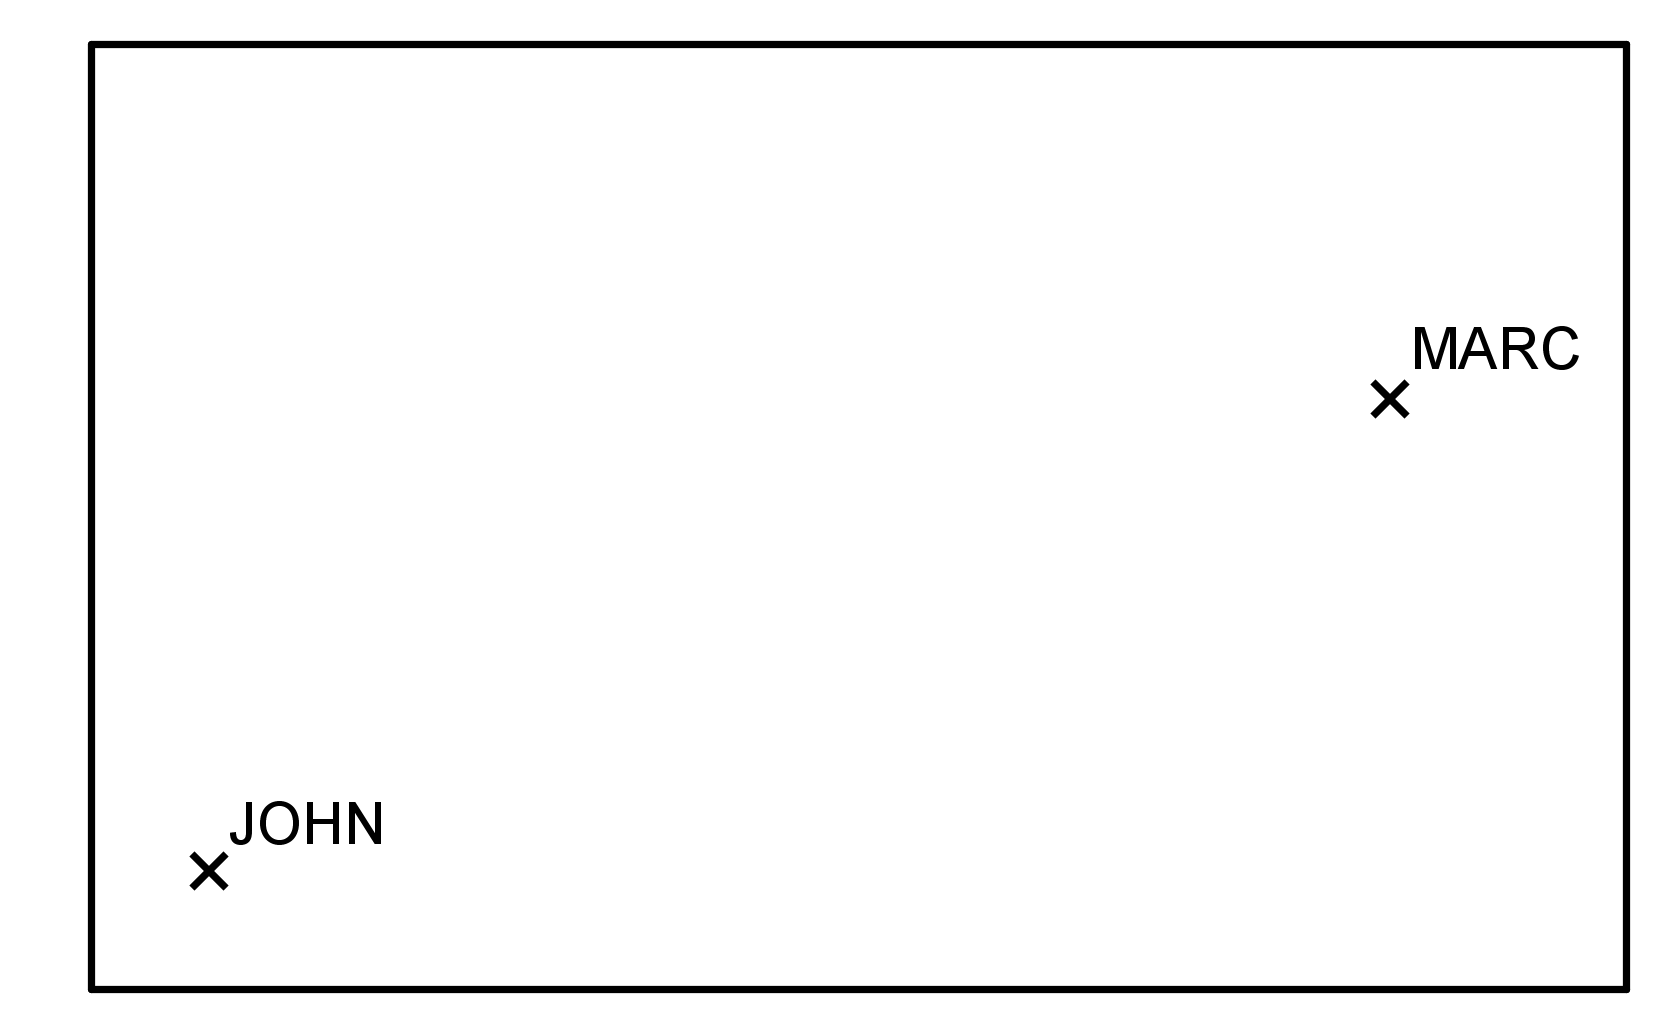
\includegraphics[width=133mm]{images/ex5.png} &
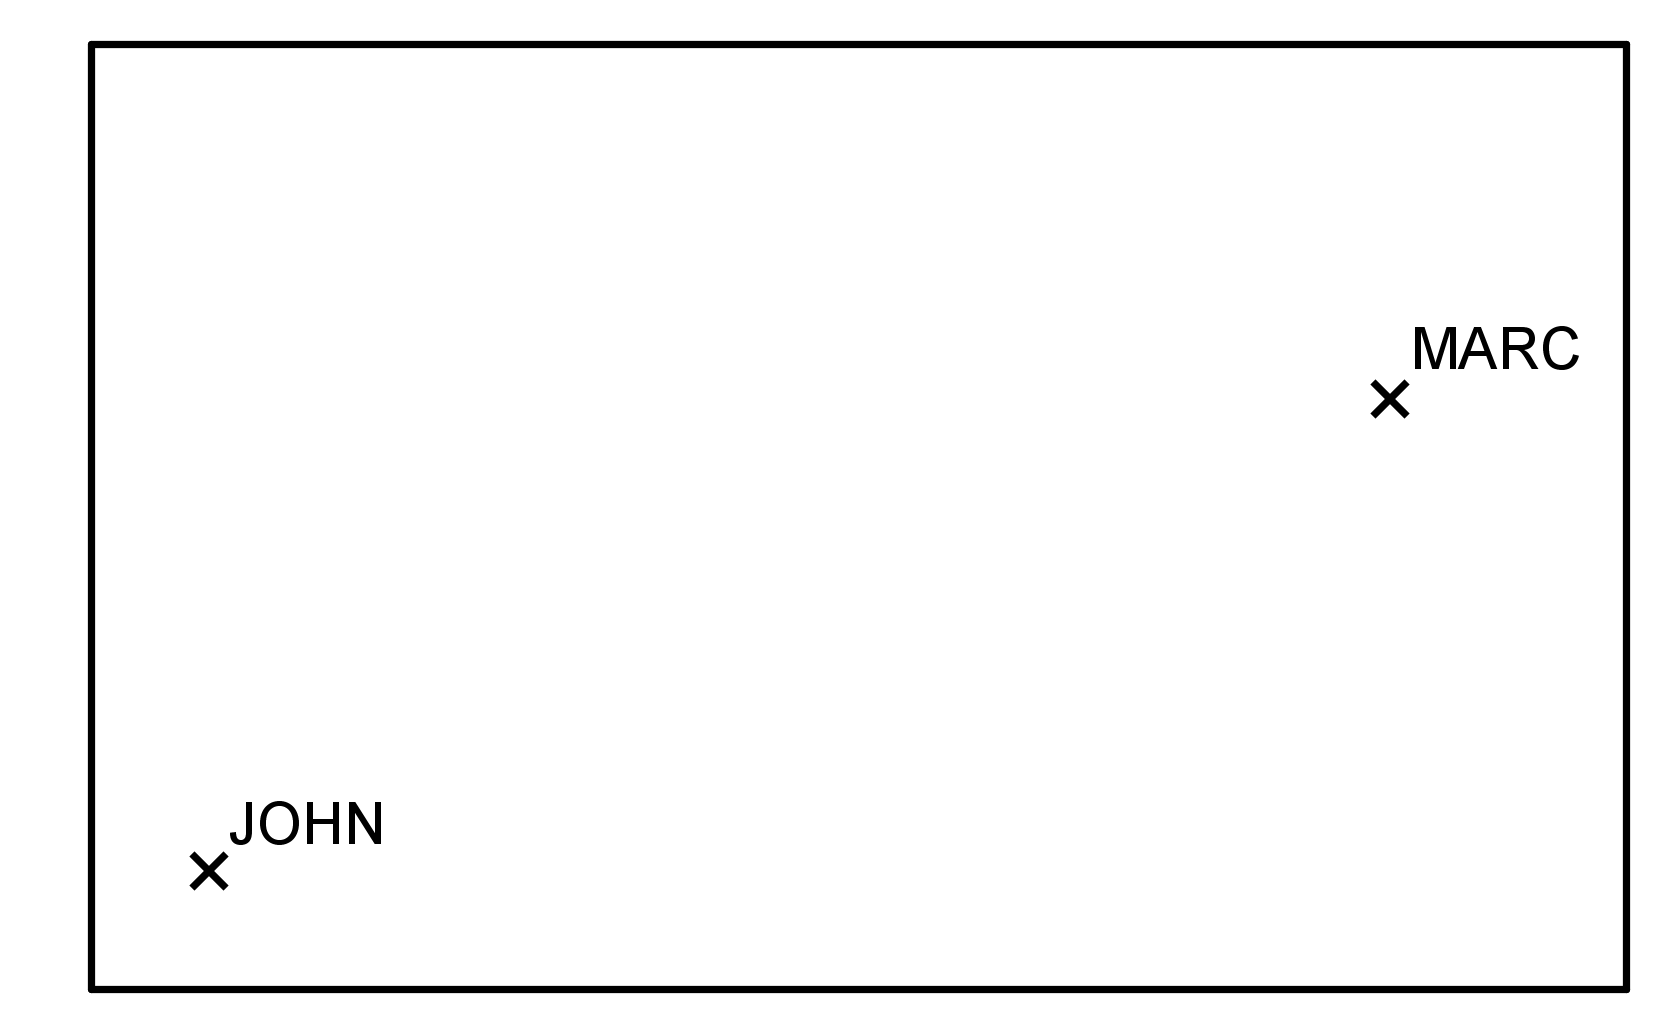
\includegraphics[width=133mm]{images/ex5.png} \\

\qquad & \qquad \\


\qquad & \qquad \\

\qquad & \qquad \\

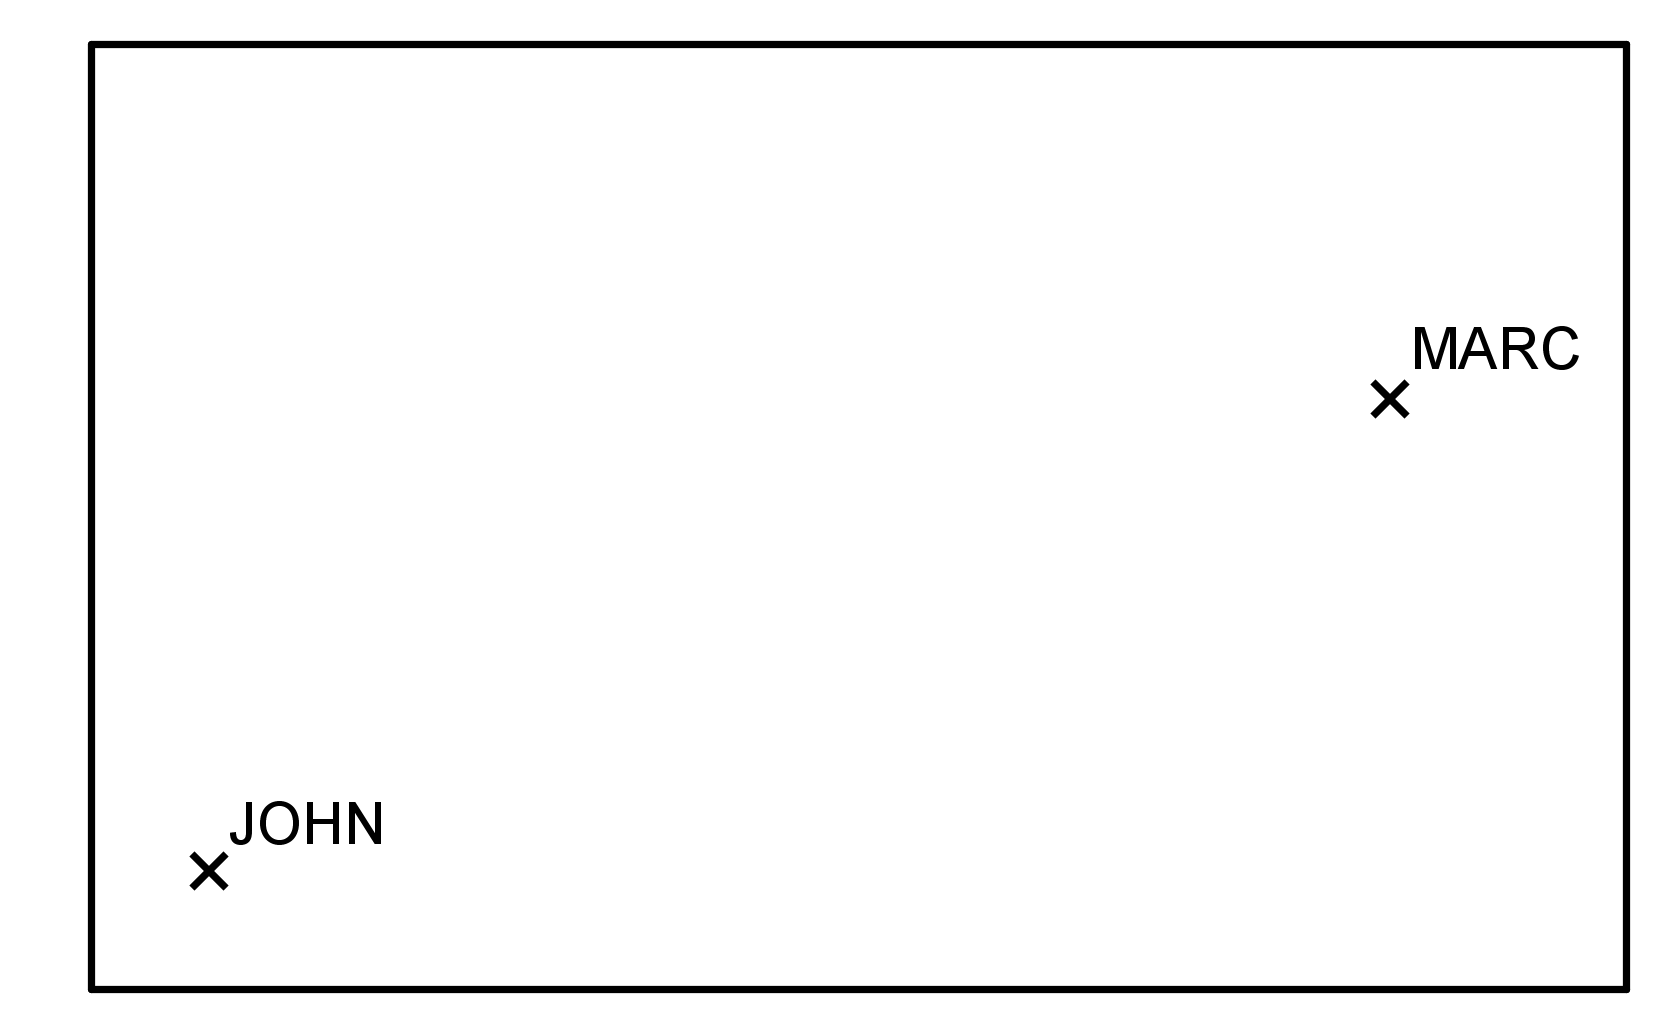
\includegraphics[width=133mm]{images/ex5.png} &
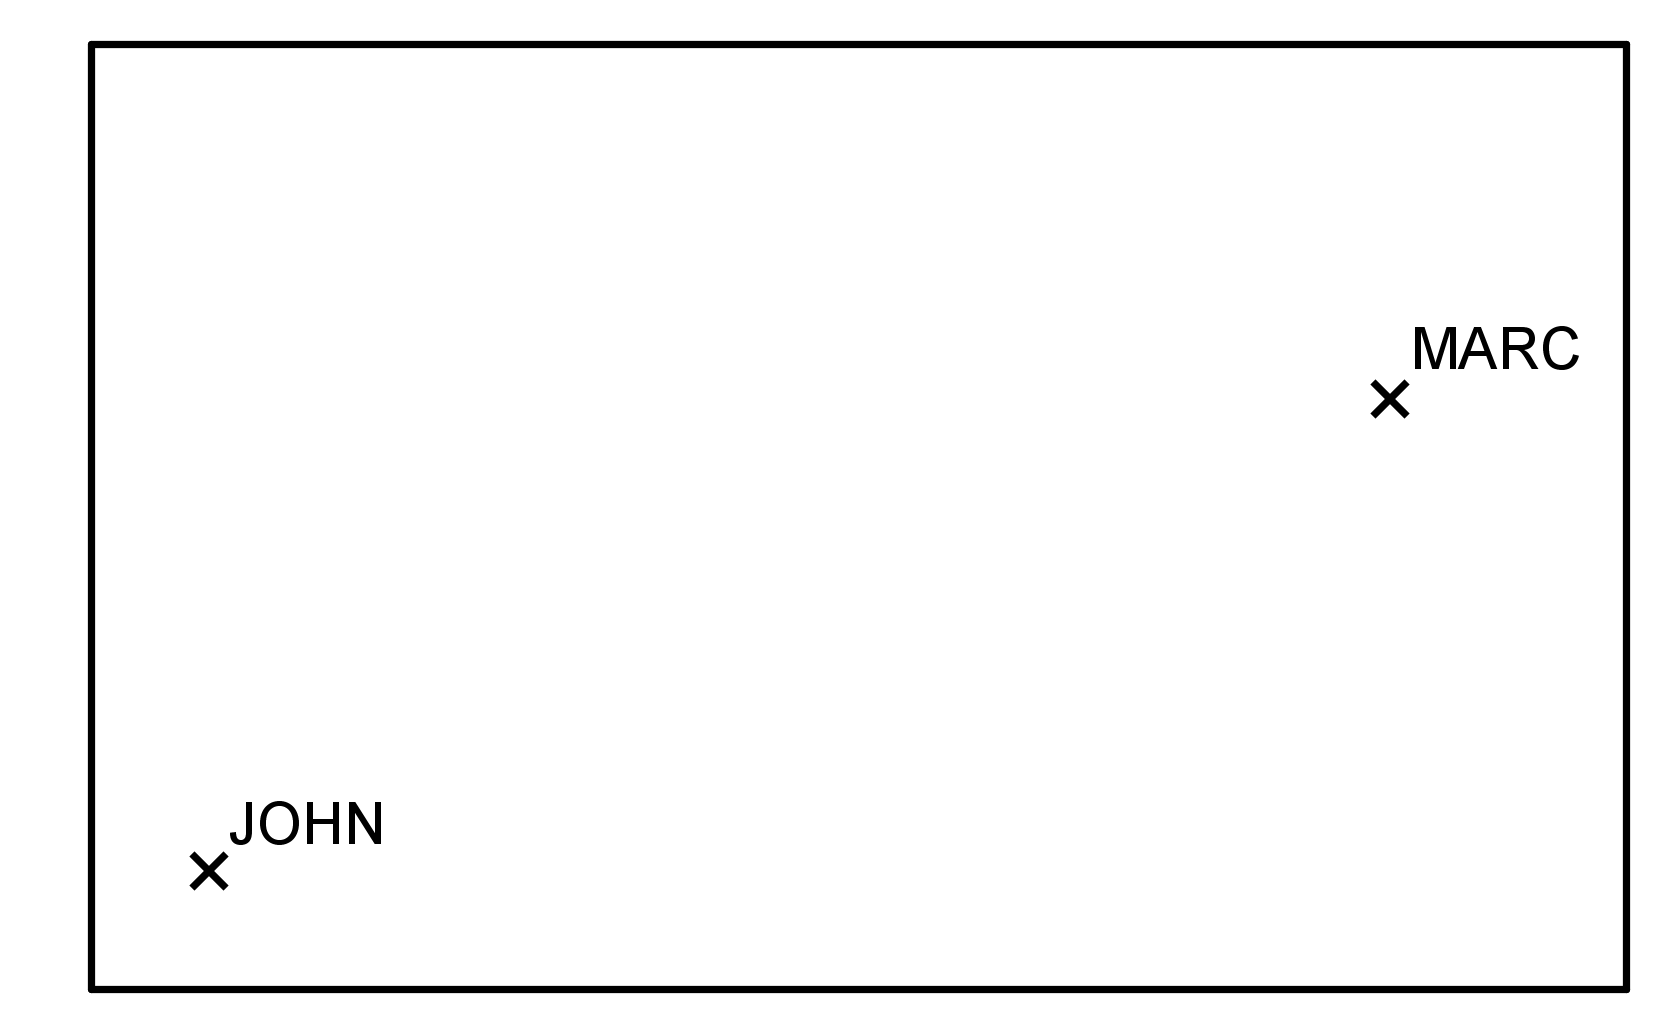
\includegraphics[width=133mm]{images/ex5.png} \\
\end{tabular}
 \end{center}
 
\end{landscape}


\end{document}
